\documentclass{article}
%\url{https://tex.stackexchange.com/q/410096/86}
\usepackage{tikz}
\usetikzlibrary{hobby,knots}

\pgfdeclarelayer{back}
\pgfsetlayers{back,main}

\begin{document}

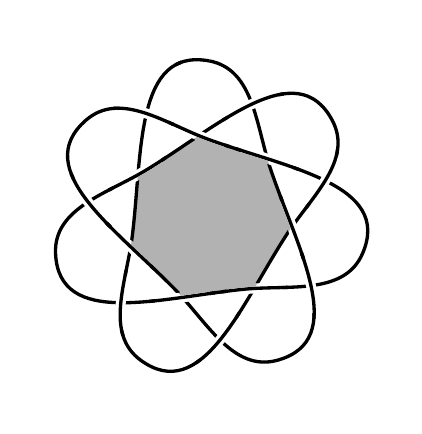
\begin{tikzpicture}[use Hobby shortcut]

\begin{scope}[blend group=darken]

\begin{scope}[blend group=normal,even odd rule]
\clip (0,0) circle[radius=1.07];
\fill[black!30!white, save Hobby path={knot}] ([closed]90:2) foreach \k in {1,...,7} 
   { .. (90-360/7+\k*1080/7:1) .. (90+\k*1080/7:2) } (90:2);
\end{scope}

\begin{scope}[blend group=normal]
\begin{knot}[
  consider self intersections=true,
  ignore endpoint intersections = false,
  flip crossing/.list={1,7,6,11,10, 13, 15, 2}
]
   \strand[very thick] ([closed]90:2) foreach \k in {1,...,7} { .. (90-360/7+\k*1080/7:1) .. (90+\k*1080/7:2) } (90:2);
\end{knot}
\end{scope}

\end{scope}
\end{tikzpicture}
\end{document}
